\startchapter{Background Material}
\label{chapter:background}

\newlength{\savedunitlength}
\setlength{\unitlength}{2em}
This chapter provides a short summary of the material which is relevant to the subject of this research. Starting with the concepts underlying 
implicit and deformable tissue modeling and an outline of continuum mechanics and finite element concepts, the chapter will conclude by reviewing closely related 
deformable models presented in the litrature. 

\section{Implicit Modeling}
\label{sec:implicitmodelingintro}
Implicit surfaces are two-dimensional, geometric shapes that exist in three-dimentional space; they can be defined based on discrete data, 
radial basis functions, offset surfaces, algebraic surfaces, level sets or distance fields to skeletal geometric primitives \cite{Bloomenthal1997}.
Independently of its origin, an implicit surface can be defined as a level-set function $F:\mathbb{R}^3 \rightarrow \mathbb{R}$ where the surface 
and the volume can be defined as following:

\begin{equation}
S = \left\{M = (x,y,z) \in \mathbb{R}^3 | F(x,y,x) = c\right\}
\end{equation}

\begin{equation}
V = \left\{M = (x,y,z) \in \mathbb{R}^3 | F(x,y,x) \geq c\right\}
\end{equation}

$c$ is a constant and is called the \textit{iso-value} which is set to $0.5$ in our system. For each point in space if the field is greater than
$c$ the point is considered inside the model otherwise outside. 

Most of the primitives used in the \blob are built from geometric skeletons, which are incorporated in many implicit modeling software packages 
such as BlobTree.net \cite{de2008blobtree} or ShapeShop \cite{Schmidt2006}. They are ideally suited to prototype shapes of arbitrary topology 
\cite{Bloomenthal1997}. In general these works conclude that the use of skeletal primitives can lead to a simple and intuitive user modelling 
methodology. The basic building block of a skeletal primitive is a skeleton $S$. To create a skeletal primitive the distance-field $dS$ of the 
volume encapsulating the shape has to be computed as described in \cite{Barbier2004}. The distance field is a volume of scalar values which is 
not bounded as the distance itself can be infinitely large.

By modifying $dS$ with a field function $g$, it can be bound to a finite range. Usually the function maps the distances to the range $[0, 1]$, 
where the field has values of 1 at the skeletons and 0 after a certain distance to the skeleton (usually at distance 1). A discussion of field 
function appears in \cite{shirley2009graphics}. Skeletal implicit primitives are combined using binary operators, which are applied pair wise to 
field-values f, and represented by a node in the BlobTree, whose children are either primitives or operators themselves.
Field values are computed for the child-nodes and combined to yield a new value according to the operator type. This makes it possible to go beyond 
the classical Boolean operators, and define general blend operators that e.g. create smooth transitions between shapes. The most common operator 
that creates a smooth transition between several values is called the summation blend \cite{Bloomenthal1997}:

\begin{equation}
F_A(x, y, z)=\sum_{i=1}^{i=N_A}F_i(x, y, z)
\end{equation}

Where an implicit model $A$ is generated by summing the influences of $N_A$ skeletal elements: 
The field value due to an skeletal element at a point in 3D space is computed as filtered distance to its skeleton 
where the filter function (i.e. falloff function) is defined as follows \cite{Wyvill1999}: 

\begin{equation}
g_\mathrm{wyvill}(x)= \left\{ \begin{array}{rl}
 1 &\mbox{ if $x\leq0$} \\
 (1-x^2)^3 &\mbox{ if $0<x<1$}\\
  0 &\mbox{ if $x\geq1$}  
  \end{array} \right.
\label{eq:WyvillFunc}
\end{equation}

In equation \ref{eq:WyvillFunc}, $x$ is clamped to the range $[0,1]$. This polynomial smoothly decreases from 1 to 0 over the valid range, with zero
tangents at each end. An important property of this skeletal primitive definition is that the scalar field is \textit{bounded}, meaning that $f=0$
outside some sphere with finite radius. Bounded fields guarantee local influence, preventing changes made to a small part of a complex model from
affecting distant portions of the surface. Local influence preserves a \textquotedblleft principle of least surprise\textquotedblright that is critical for interactive modeling.  
Normals can be derived from gradients which are computed by evaluating 4 field values and performing a numerical approximation:

\begin{equation}
\nabla F(x,y,z)=\left\{ \begin{array}{rl}
 F(x+\delta,y,z)-f \\
 F(x, y +\delta,z)-f \\
 F(x, y, z+\delta)-f \\
  \end{array} \right. 
\label{eq:Normal}
\end{equation}

Where $f = F(x,y,z)$ is the field at point $(x,y,z)$.
% $fv = F(x,y,z)$ be the field at a point:
%$\nabla F(x,y,z)=\frac{1}{\delta}\left( F(x+\delta,y,z)-fv \right)$

Each skeletal primitive has a bounded region of influence in space. For each node in the tree an
axis-aligned bounding box is computed which is used to trivially reject those field queries that 
are outside the box. The bounding box of the entire model is computed as the union of all primitive
nodes bounding boxes.

For evaluating the field  at a point $P$ in a \blob model such as the one shown in figure (\ref{fig:CoffeeMugBlobTree}), 
the tree structure should be traversed from root to leaves recursively. Each operator combines the values of its children 
according to its type. For example, for a simple blend the values are summed. A leaf node represents a primitive,  and 
returns the value by applying equation~\ref{eq:WyvillFunc} to the distance of $P$ from the primitive.

%The right way for inserting figures
\begin{figure}[H]
\centering
  % the following command controls the width of the embedded PS file
  % (relative to the width of the current column)
  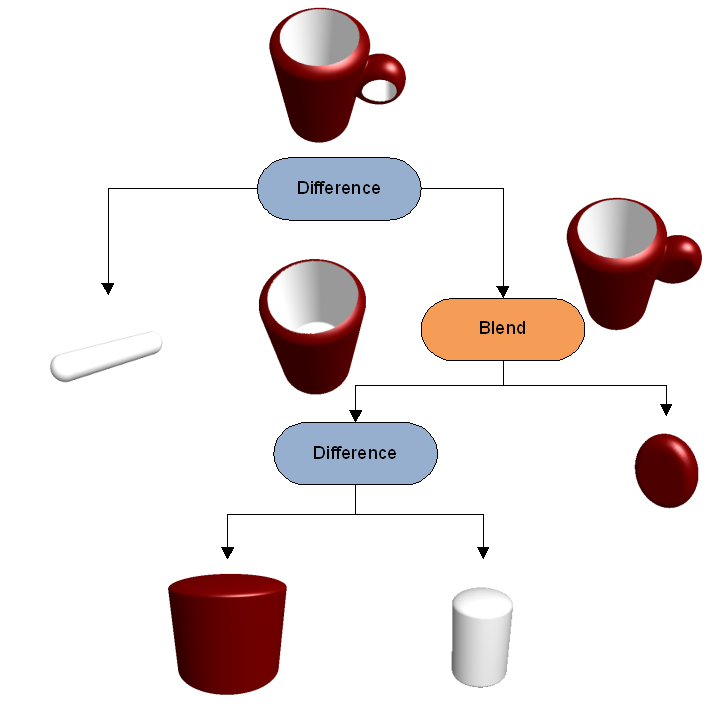
\includegraphics[width=1.0\linewidth]{figures/intro/CoffeeMugBlobTree}
  \caption{\blob structure of a coffee mug created with CSG and skeletal implicit primitives.}
  \label{fig:CoffeeMugBlobTree}
\end{figure}

%As the tree gets deeper and the number of primitives increase the computation 
For visualization purposes the \blob is queried numerous times to evaluate the field. As suggested in \cite{SWG2005} 
accelerating field computation will have a large impact on the overall surface extraction process. 

\section{Sweep Surfaces and Sketching}
Implicit primitives in our system are created from skeletons which are simple geometrical shapes such as points, line segments or 
polygons from which volumetric distance fields are created. In order to support more complex geometries \textit{Schmidt} \etal proposed the
implicit sweep objects technique where the 2D shape sketched by the user is sampled and an implicit approximation is created from 
the sample points \cite{Schmidtc}. This is done by fitting a thin-plate spline as a base shape to the sampled points using variational 
interpolation \cite{Turk1999}. One advantage of creating the base shape using variational interpolation is that the resulting implicit 
field is $C^2$ continuous, a property needed when the shape is involved in several blending operations \cite{barthe2004controllable}.

A continuous 2D scalar field is created from several field value samples $(\mathbf{m}_i, v_i)$, where $\mathbf{m}_i$ describes the 
position of the sample and $v_i$ is the desired field. The thin-plate spline used to create the variational 
implicit field $f_c(\mathbf{u})$ is defined in terms of these points weighted by corresponding coefficients $w_i$ combined with a polynomial 
$P(u) = c_1u_x +c_2u_y +c_3$.

\begin{equation}
f_c(\mathbf{u}) = \sum_{i \in N} w_i(\|\mathbf{u}-\mathbf{m}_i\|)^2ln(\|\mathbf{u}-\mathbf{m}_i\|)+P(\mathbf{u}) 
\label{eq:thinplatespline}
\end{equation}

The weights $w_i$ and coefficients $c_1$, $c_2$, and $c_3$ are found by solving a linear system defined by evaluating 
equation \ref{eq:thinplatespline} at each known solution $f_c(\mathbf{m}_i)=v_i$.
The resulting thin plate spline can then be used as the basis of several different primitives:

\begin{itemize}
 \item Inflated Objects
 \item Swept object along a trajectory
 \item Revolving object around axis
\end{itemize}

These sketched objects can then be used in the same way as the standard skeletal implicit primitives to create unique 3D shapes. Such 
unique shapes were not possible to create in previous collaborative environments, especially given this technique’s small memory footprint 
needed to transfer the information.

\section{Deformable Models}
In their survey paper Meier \etal \cite{Meier2005} presented a classification of the deformable models available for surgery 
simulation based on their applications. The main classifications are heuristic, hybric and continuum mechanical approaches.
Examples of heuristic models are: deformable splines, spring-mass models, linked volumes and tensor-mass models. 

With deformable splines, classical splines are employed to model a 3D object. They define a potential energy which is proportional
to the degree of elastic deformation. By using the lagrange method, this energy is finally minimized with respect to the displacements
enforced in some control points to obtain the corresponding deformation state. The increased number of parameters required to control
the shape and the physical properties of the models will become the bottleneck and are difficult to determine empirically. A post processing
step is also required to convert the smooth spline surface to discretized polygons for rendering. Even without this post processing stage
they are computationally very expensive. E.g. solid objects have to be modelled as hollow shells which is not lending itself very well for
volume preservation applications.

\subsection{Mass-Spring Models}
Mass spring models (MSM) are the most intuitive and most common method used in deformable object modeling.
Terzopoulos \etal \cite{terzopoulos1988modeling, terzopoulos1987elastically} was the first who introduced mass-spring systems in 
computer graphics animation systems. Provot \etal showed applications of this technique in cloth simulation \cite{provot1995deformation}
as did Baraff \etal \cite{baraff1998large}. Kahel \etal used in facial animation \cite{kahler2001geometry}. 
Gibson \etal survey reviewed many examples of mass-spring system applications \cite{Gibson1997a}. In this system the deformable object
is discretized into a network of point masses which are connected with massless springs and dampers. By adding weights and considering
constant coefficient $k_s$ the elastic force is obtained by:

\begin{equation}
 \boldsymbol{f}^s_i = \sum_{j \in N(\boldsymbol{x}_i)} k_s w_{ij}(\boldsymbol{x}_{ij})(1-\frac{l^0_{ij}}{\| \boldsymbol{x}_{ij} \|})
\end{equation}

In this setup:

\begin{itemize}
 \item $\boldsymbol{x_{ij}} = \boldsymbol{x}_j - \boldsymbol{x}_i$ where $\boldsymbol{x}_i$ is the position of node $i$, 
 \item $l^0_{ij}$ is the initial spring length between node $i$ and node $j$,
 \item $N(\boldsymbol{x_i})$ is the set of neighbors of node $i$ and $w_{ij}$ is the weight of $j$th neighbor of node $i$.
\end{itemize}

The damping force in this setup is given by:

\begin{equation}
 \boldsymbol{f}^d_i = \sum_{j \in N(\boldsymbol{x}_i)} k_d w_{ij} \frac{\boldsymbol{v}^\tau_{ij} \boldsymbol{x}_{ij} }{\|\boldsymbol{x}_{ij} \|} \boldsymbol{x}_{ij}
\end{equation}
where $\boldsymbol{v}_i$ is the velocity of node $i$ and $\boldsymbol{v}_{ij} = \boldsymbol{v}_j - \boldsymbol{v}_i$.

\subsection{Linked Volumes}
\label{sec:linkedvolumes}
The ideas in MSM can be extended to volumetric modeling by discretizing the entire volume of a deformable model into evenly spaced cubic elements.
The total mass of the model is distributed at the centers of these cubes. The cubes are interconnected with their neighbors using springs and dampers
\cite{gibson1997simulating}. One of the disadvantages of this approach is its increased computational cost due to the higher number of nodes and
their increased connectivity. In order to control the computational cost for large models the resolution of the discretization should be lowered 
which will lead to unrealistic deformations. For rendering purposes auxilary surface representations should be used such as surface maps. 
Increasing the number of elements slows down the propagation of deformations. The benefit of this approach is that complex interactions such as
cutting, carving, joining, or tearing can easily be represented by simply eliminating or adding links between elements.


\subsection{Mass Tensor Model}
Using this technique the entire interior of the model is discretized into tetrahedrons. Points masses and springs are 
being placed at the respective tetrahedral vertices and edges \cite{de1999modeling}. The performance of this model is comparable to that of the 
linked volumes describe earlier in section \ref{sec:linkedvolumes}. Cutting models created with this techniques is a challenge since even when
minimizing the number of newly created tetrahedrons in such a situation the corresponding increase of nodes in significant and directly hits the
performance of the system. The performance of the model depends on the resolution of the mesh in this case \cite{picinbono2000real}. 


\section{Continuum Mechanics Concepts} 
Continuum biomechanics for soft tissue simulation deals with the movement of soft materials when subjected to applied forces \cite{Sifakis2012}. 
The motion of a continuous and deformable solid can be described by a continuous displacement field resulting from a set of 
forces acting on the solid body. A displacement \textit{field} implies a continuous variation of displacement with position. 
The continuous displacement field can be time-independent or time-dependent. The initial unloaded state of material is referred to 
as the \textit{reference} or \textit{undeformed} state as the displacements are zero everywhere. The material then reconfigures due to 
applied loads and reaches an equilibrium state referred to as \textit{deformed} state. The concepts of \textit{strain}, a measure of length
change or displacement gradient, and \textit{stress}, the force per unit area on an infinitesimally small plane surface within the material, 
are of fundamental importance for continuum biomechanics of soft tissues. 

The formulation of models in continuum mechanics consists of three parts:

\begin{enumerate}
 \item Kinematics: Geometric description of the deformation
 \item Dynamics: A formulation of the equations of motion
 \item Constituitive formulation: Description of the material properties
\end{enumerate}

\section{Deformation map and deformation gradient}
Our initial objective is to provide a concise mathematical description of the deformation that an elastic body has sustained. This formulation will 
lay the foundation for appropriate representations of other physical properties such as force and energy. We begin by placing the undeformed elastic 
object in a coordinate system, and denote by $\Omega$ the volumetric domain occupied by the object. This domain will be referred to as the reference 
(or undeformed) configuration, and we follow the convention that capital letters $\vec{X} \in \Omega$ are used when referring to individual material
points in this undeformed shape. Note that the precise position and orientation of the undeformed elastic body within the reference space is not important 
and can be chosen at will, as long as the shape of the object corresponds to a rest configuration

When the object undergoes deformation, every material point $\vec{X}$ is being displaced to a new deformed location as seen in figure 2.1 (top) which is, 
by convention, denoted by a lowercase variable $\vec{x}$. The relation between each material point and its respective deformed location is captured by 
the deformation function $\vec{\phi} : \mathbf{R}^3 \rightarrow \mathbf{R}^3$ which maps every material point $\vec{X}$ to its respective deformed 
location $\vec{x}=\vec{\phi}(\vec{X})$.

An important physical quantity derived directly from $\vec{phi}(\vec{X})$, whose utility will become apparent in the next sections, is the deformation 
gradient tensor $\mathbf{F} \in \mathbf{R}^{3 \times 3}$. If we write $\vec{X} =(X_1,X_2,X_3)^T $ and 
$\vec{\phi}(\vec{X})=(\phi_1(\vec{X}), \phi_2(\vec{X}), \phi_3(\vec{X}))^T$ for the three components of the vector-valued function $\vec{\phi}$,
the deformation gradient is written as: 

\begin{equation}
 \mathbf{F} := \frac{\partial(\phi_1, \phi_2, \phi_3)}{\partial (X_1, X_2, X_3)}= 
 \left(\begin{array}{ccc} 
      \partial \phi_1/\partial X_1 & \phi_1/\partial X_2 & \phi_1/\partial X_3 \\
      \partial \phi_2/\partial X_1 & \phi_2/\partial X_2 & \phi_2/\partial X_3 \\
      \partial \phi_3/\partial X_1 & \phi_3/\partial X_2 & \phi_3/\partial X_3 
      \end{array} \right)
\end{equation}



or, in index notation $F_{ij} = \phi_{i,j}$. That is, F is the Jacobian matrix of the deformation map. Note that, in general, $F$ will be spatially varying 
across $\Omega$; in the next sections we will use the notation $F(\vec{X})$ if such dependence needs to be made explicit.

\section{Strain energy}
When a deformable tissue undergoes some deformation the energy will be accumulated in the object which is called \textit{strain energy}: $E[\phi]$ (We 
follow the same notation given in \cite{Sifakis2012}) The \textit{strain energy} is fully determined by the deformation map of a given configuration.
One of the characteristics of \textit{hyperelastic} materials is that their \textit{strain energy} is independent of the prior deformation history 
of the object. This property is closely related to the fact that the elastic forces of the \textit{hyperelastic} materials are \textit{conservative}.
The total work done by the internal elastic forces in a deformation path depends solely on the initial and final configurations and not the path itself.

When applying forces on a deformable tissue, different regions of the tissue will undergo shape changes of different severity. Thus, in order to compute the 
strain energy we start from a local view of the deformations. An \textit{energy density} function $\Psi[\phi; \vec{X}]$ measures the strain energy 
\textit{per unit of undeformed volume} on an infinitesimal domain $dV$ around the material point $\vec{X}$. The total energy of the deforming body is then 
computed by integrating the energy density function over the entire domain $\Omega$:

\begin{equation}
  E[\phi]=\int_\Omega\Psi[\phi;\vec{X}]d\vec{X}
\end{equation}

%todo: Add some examples for the strain energy formula

We survey a number of different simulated materials and describe how their physical properties are encoded in their respective governing equations. The 
\textit{constitutive model} is the mathematical description of the physical characteristics of a given material and includes the equations that relate
stimuli (e.g. deformations) to the material response which can be the force, stress or energy they trigger. 

\section{Strain Computation}
In principle, an explicit formula that relates $\Psi$ and $\vec{F}$ would be perfectly adequate as a constitutive equation. The challenge, with designing
constitutive models in this fashion is that using the raw elements of the matrix $F$ can be a very unintuitive way to argue about the flavor and severity
of a given deformation. It is possible that a certain material's response is dominated by its affinity for volume conservation, while a different material
might prioriatize resistance to shear. Metrics such as ``The ratio of the volumetric expansion'' or ``the shear angle'' would be much more effective in 
expressing the severity of the types of deformation that are most relevant to such materials. As a consequence, it is common for the design process for 
constitutive models to define certain intermediate quantities such as strain measures and invariants which are derived from F, yet capture the specific 
traits of the deformation that the energy or stress values depend on more concisely than the deformation gradient itself.


A strain measure is intended to be a quantitative descriptor for the severity of a given deformation, i.e. a way to gauge how far this configuration is 
from a rest configuration. For this reason, although strain measures are derived from the deformation gradient, they strive to retain as much information 
from it that is relevant to assessing deformation magnitude while disregarding any information contained in it that is unrelated to shape change. 
The deformation gradient contains all the information necessary to determine how a small neighborhood of a material point deforms. One would like, 
however, to distinguish between two important cases, namely, those in which the neighborhood of a point has just undergone a rigid motion and, on the other 
hand, those in which the neighborhood has undergone a true change of shape or of size. In the first case, the deformation gradient would correspond to a 
pure rotation. Mathematically, this phenomenon manifests itself in the fact that the matrix representing the deformation gradient $\mathbf{F}$ is a so called
\textit{orthogonal} matrix. An orthogonal matrix $\mathbf{R}$ is characterized by the property that its inverse, $\mathbf{R}^{-1}$, is equal to its transpose,
$\mathbf{R}^T$. For a pure rotation (as opposed to a reflection) the determinant of an orthogonal matrix is equal to +1 (instead of -1 for a combined rotation
and reflection). The question is: given an arbitrary $\mathbf{F}$, is it possible to separate the part that corresponds to a pure rotation from the part 
representing a true change of shape and/or of size? The answer to this question is given by a remarkable theorem in algebra known as the 
\textit{polar decomposition theorem}. It asserts that every non-singular matrix $\mathbf{F}$ can be uniquely decomposed into the product of an orthogonal 
matrix $R$ and a positive definite symmetric matrix $U$, as follows:

\begin{equation}
\mathbf{F} =  \mathbf{R}\mathbf{U}
\end{equation}

A positive definite symmetric matrix (namely, one with all positive eigenvalues) can be shown to represent pure elongations or contractions along three 
mutually perpendicular axes (the so-called \textit{principal axes}) \cite{fung2001classical}.

Consider the Green strain tensor $\mathbf{E} \in \mathbf{R}^{3\times 3}$, defined as:

\begin{equation}
\mathbf{E} = \frac{1}{2}(\mathbf{F}^T\mathbf{F}-\mathbf{I}).
\end{equation}

These axes, defined in the point at the reference configuration, are the \textit{eigenvectors} of the symmetric matrix:

\begin{equation}
\mathbf{C} =  \mathbf{F}^T\mathbf{F}
\end{equation}

known as the \textit{right Cauchy-Green tensor}. It is related to $\textbf{U}$ by the equation $\mathbf{C}=\mathbf{U}^2$.
From the preceding considerations, it follows that the neighborhood of a material point will undergo a pure rotation if, 
and only if, $\mathbf{C}=\mathbf{U}=\mathbf{I}$. Otherwise, there willl be a genuine change of size and/or shape. 


It is convenient, therefore, to introduce the following measure of \textit{strain}, sometimes called the \textit{Lagrangian 
strain tensor}: 


\begin{equation}
\mathbf{E} = \frac{1}{2}(\mathbf{C} - \mathbf{I})
\end{equation}

This tensor has the property of vanishing if, and only if, there is no strain (change of shape and/or size) at the points in question.
Again there are no limitations whatsoever to the magnitude of the derivatives of the displacements used to calculate the Lagrangian
strain tensor. 


\section{Linear Elasticity}
The simplest practical constitutive model is linear elasticity, defined in terms of the strain energy density as:

\begin{equation}
\label{eq:linearelasticity}
 \Psi(\mathbf{F}) = \mu\boldsymbol{\epsilon}:\boldsymbol{\epsilon} + \frac{\lambda}{2}tr^2(\boldsymbol{\epsilon})
\end{equation}

where $\boldsymbol{\epsilon}$ is the small strain tensor and $\mu$, $\lambda$ are the \textit{Lame coefficients}, which are related to
the material properties of \textit{Young's modulus k} (a measure of stretch resistance) and \textit{Poisson's ratio} $\nu$ (a 
measure of incompressibility) as:

\begin{align*}
\mu=\frac{k}{2(1+\nu)} \hspace{10 mm} \lambda=\frac{k\nu}{(1+\nu)(1-2\nu)}
\end{align*}

The relation between the Piola stress $\mathbf{P}$ and $\mathbf{F}$ can be derived as follows:

\begin{gather*}
\delta \boldsymbol{\epsilon} =\frac{1}{2}(\delta\mathbf{F} + \delta\mathbf{F}^T)=Sym\left\{\delta\mathbf{F}\right\}  \\
\boldsymbol{\epsilon}:\delta\boldsymbol{\epsilon}=\boldsymbol{\epsilon}:Sym\left\{\delta\boldsymbol{F}\right\}=\epsilon:\delta\boldsymbol{F} \hspace{10 mm}
tr(\delta\boldsymbol{\epsilon})=\boldsymbol{I}:Sym\left\{\delta\boldsymbol{F}\right\}=\boldsymbol{I}:\delta\boldsymbol{F} \\
\delta\Psi=2\mu\boldsymbol{\epsilon}:\delta\boldsymbol{\epsilon}+\lambda tr(\boldsymbol{\epsilon})  tr(\delta\boldsymbol{\epsilon})=[2\mu\boldsymbol{\epsilon}+\lambda tr(\boldsymbol{\epsilon})]\boldsymbol{I}:\delta\boldsymbol{F}\\
Thus \hspace{10 mm} \boldsymbol{P}=2\mu\boldsymbol{\epsilon}+\lambda tr(\boldsymbol{\epsilon})\boldsymbol{I}
\end{gather*}

after one final substitution for $\boldsymbol{\epsilon}$ and a few algebraic reductions:

\begin{align*}
  \boldsymbol{P}(\boldsymbol{F})=\mu(\boldsymbol{F} + \boldsymbol{F}^T-2\boldsymbol{I})+\lambda tr(\boldsymbol{F} - \boldsymbol{I})\boldsymbol{I}
\end{align*}

These expressions allow us to make the following observations:

\begin{itemize}
 \item The stress $\boldsymbol{P}$ is a \textit{linear} function of the deformation gradient. As a result, this constitutive model is characterized by a significantly
lower computational cost that other, nonlinear materials. 

\item Since the small strain tensor was designed to be accurate exclusively in a small deformation scenario, it is more appropriate to use linear elasticity when the magnitude
of motion is small. For example, a rigid motion $\vec{\phi}(\vec{X})=\boldsymbol{R}\vec{X}+\vec{t}$ would generally produce a non-zero strain 
$\epsilon = \frac{1}{2}(\boldsymbol{R}+\boldsymbol{R}^T)-\boldsymbol{I}$ and ultimately a non-zero stress, even though no shape change has taken place. 
\end{itemize}

\section{St. Venant-Kirchhoff model}
With the understanding that the small strain tensor is a mere approximation of the rotationally invariant Green strain $\boldsymbol{E}$, it 
makes sense to attempt an improvement of the linear elasticity model by using $\boldsymbol{E}$ in the place of $\boldsymbol{\epsilon}$ is equation
 (\ref{eq:linearelasticity}):

 \begin{equation}
 \Psi(\mathbf{F}) = \mu\boldsymbol{E}:\boldsymbol{E} + \frac{\lambda}{2}tr^2(\boldsymbol{E})
 \end{equation}

This constitutive model is recognized as \textit{St. Venant-Kirchhoff} material, and is the first truely nonlinear material we will examine. The first
Piola-Kirchhoff stress tensor can be computed via a process similar to the one followed for linear elasticity:

\begin{gather*}
  \delta\boldsymbol{E}=\frac{1}{2} (\delta\boldsymbol{F}^T\boldsymbol{F}+ \boldsymbol{F}^T\delta\boldsymbol{F})=Sym\left\{\boldsymbol{F}^T\delta\boldsymbol{F}\right\}\\
  \boldsymbol{E}:\delta\boldsymbol{E}=\boldsymbol{E}:\left\{\boldsymbol{F}^T\delta\boldsymbol{F}\right\}=\left\{\boldsymbol{FE}\right\}:\delta\boldsymbol{F}
  \hspace{10 mm} tr(\delta\boldsymbol{E})=\boldsymbol{I}:\left\{\boldsymbol{F}^T\delta\boldsymbol{F} \right\}=\boldsymbol{F}:\delta\boldsymbol{F}\\
  \delta\Psi=2\mu\boldsymbol{E}:\delta\boldsymbol{E}+\lambda tr(\boldsymbol{E})tr(\delta\boldsymbol{E})=\boldsymbol{F}\left[2\mu\boldsymbol{E}+\lambda tr(\boldsymbol{E}) \boldsymbol{I} \right]:\delta\boldsymbol{F}
\end{gather*}


\begin{equation}
\label{eq:venantkirchhoff}
Thus \hspace{10 mm} \boldsymbol{P}(\boldsymbol{F})=\boldsymbol{F}\left[2\mu\boldsymbol{E}+\lambda tr(\boldsymbol{E})\boldsymbol{I}\right]. 
\end{equation}

This is a rotationally invariant model; deformations that differ by a rigid body transformation are guaranteed to have the same strain energy. As a 
consequence a St. Venant-Kirchhoff material exhibits plausible material response in many large deformation scenarios where linear elasticity would 
not be applicable. Equation (\ref{eq:venantkirchhoff}) indicates that stress is a 3rd degree polynomial function of the components of $\boldsymbol{F}$; 
after discretization, nodal forces will likewise be expressed as cubic polynomials of nodal positions.
Although the St. Venant-Kirchhoff model offers significant benefits over a linear elastic model, its scope is limited to a certain degree due to its 
poor resistance to forceful compression: as a St. Venant-Kirchhoff elastic body is compressed, starting from its undeformed configuration, it reacts 
with a restorative force which initially grows with the degree of compression. However, once a critical compression threshold is reached 
($\approx 58\%$ of undeformed dimensions, when compression occurs along a single axis) the strength of the restorative force reaches a maximum. Further
compression will be met with decreasing resistance, in fact the restorative force will vanish as the object is compressed all the way down to zero volume 
(an indication of this is that when $\boldsymbol{F} = 0$ we also have $\boldsymbol{P} = 0$). Continued compression past the point of zero volume (forcing the material to invert) will 
then create a restorative force that pushes the body towards complete inversion (reflection) along one or more axes. In practical computer simulation 
examples this behavior often manifests itself as a tendency of the material to locally tangle and invert itself when subjected to strong compressive forces 
or kinematic constraints.

 
\section{Corotated linear elasticity}
The use of the quadratic Green strain in the St. Venant-Kirchhoff guaranteed the rotational invariance of the constitutive model. At the same time, 
the increased complexity inherent in highly nonlinear materials leads to unintended side effects, such as the non-physical zero stress configurations 
of St. Venant-Kirchhoff materials under extreme compression. Corotated linear elasticity is a constitutive model that attempts to combine the simplicity 
of the stress-deformation relationship in a linear material with just enough nonlinear characteristics to secure rotational invariance.
Using the polar decomposition $\boldsymbol{F} = \boldsymbol{R}\boldsymbol{S}$ we construct a new strain measure as
$\boldsymbol{\epsilon}_c = \boldsymbol{S} − \boldsymbol{I}$, which is linear on the symmetric tensor $\boldsymbol{S}$ obtained by factoring away
the rotational component of $\boldsymbol{F}$. Replacing the small strain tensor in equation (\ref{eq:linearelasticity}) we obtain the energy for corotational 
elasticity:

\begin{equation}
\label{eq:CorotatedEnergyDensity}
  \Psi(\boldsymbol{F})=\mu\boldsymbol{\epsilon}_c:\boldsymbol{\epsilon}_c+\frac{\lambda}{2} tr^2(\boldsymbol{\epsilon}_c)=
  \mu\|\boldsymbol{S} - \boldsymbol{I} \|^2_F+(\lambda/2)tr^2(\boldsymbol{S}-\boldsymbol{I})
\end{equation}

which can be equivalently written in any of the following ways:

\begin{align}
\label{eq:CorotatedEnergyDensitySVD}
\Psi(\boldsymbol{F})=\mu\|\boldsymbol{F} - \boldsymbol{R}\|^2_F+(\lambda/2) tr^2(\boldsymbol{R}^T\boldsymbol{F}-\boldsymbol{I}) \nonumber \\
\Psi(\boldsymbol{F})=\mu\|\boldsymbol{\Sigma} - \boldsymbol{I} \|^2_F+(\lambda/2) tr^2(\boldsymbol{\Sigma} - \boldsymbol{I})
\end{align}

where $\Sigma$ is the diagonal matrix with the singular values of $\boldsymbol{F}$, from the Singular Value Decomposition 
$\boldsymbol{F} = \boldsymbol{U\Sigma V}^T$. We can show that the 1st Piola-Kirchhoff stress tensor for corotated linear elasticity is given by:
 
%(\boldsymbol{F})=
%\boldsymbol{R} \left[ 2\mu\boldsymbol{\epsilon}_c \right]
 
\begin{gather*}
\boldsymbol{P}(\boldsymbol{F})=\boldsymbol{R} \left[ 2\mu \boldsymbol{\epsilon}_c + \lambda tr(\boldsymbol{\epsilon_c}) \boldsymbol{I} \right]=
\boldsymbol{R} \left[ 2\mu (\boldsymbol{S - I}) + \lambda tr(\boldsymbol{S - I}) \boldsymbol{I} \right] \\
= 2 \mu (\boldsymbol{F-R}) + \lambda tr(\boldsymbol{R}^T\boldsymbol{F} - \boldsymbol{I})\boldsymbol{R}
\end{gather*}

The motivation behind corotational elasticity is to mimic what linear elasticity would have been, if the undeformed configuration had been rotated in the same way
as encoded in the rotational factor $\boldsymbol{R}$ from the polar decomposition. In situations where the value of $\boldsymbol{R}$ varies across the domain, 
making the transition from linear to corotated elasticity is more complex than a change of variables due to a constant rotation of the undeformed configuration. 
From a computational cost perspective, the overhead of corotated vs. linear elasticity includes the cost of the polar decomposition, and the need to employ nonlinear
solvers for certain types of simulation. 

\section{Isotropic Materials}
The two mentioned constitutive material models so far have been constructed to be rotationally invariant. This property can be formally defined using a pair of 
deformation maps $\vec{\phi_1}(\vec{X})$ and $\vec{\phi_2}(\vec{X})$, that differ only by a rigid transform, specifically:

\begin{equation}
\label{eq:rigidbodytransform}
 \vec{\phi_2}(\vec{X}) = \boldsymbol{R} \vec{\phi_1}(\vec{X}) + \vec{t}, \hspace{5mm} \text{where $\boldsymbol{R}$ is a $3\times 3$ rotation matrix}
\end{equation}

A constitutive model is rotationally invariant if and only if it guarantees that the strain energy will satisfy $E\left[ \phi_1 \right] = E\left[ \phi_2 \right]$
for any such deformation pair. An equivalant definition can be provided for the hyperelastic materials based on the strain energy density function. 
After computing the gradients we can see that any two deformations that satisfy equation (\ref{eq:rigidbodytransform}) will have deformation gradient related as
$\boldsymbol{F}_2=\boldsymbol{R}\boldsymbol{F}_1$. The energy density associated with these deformations must satisfy $\Psi(\boldsymbol{F}_1)=\Psi(\boldsymbol{F}_2)$,
leading to the following equivalant definition of rotational invariance:\\

\textbf{Definition:} A hyperelastic constitutive model is \textit{rotationally invariant} if and only if the energy density satisfies

\begin{gather*}
  \Psi(\boldsymbol{RF})=\Psi(\boldsymbol{F})
\end{gather*}

for any value of the deformation gradient $\boldsymbol{F}$ and any $3 \times 3 $ rotation matrix $\boldsymbol{R}$.
One of the consequences of this definition is that the strain energy in rotationally invariant models can be written
as a function of the symmetric factor $\boldsymbol{S}$ from the polar decomposition of $\boldsymbol{F} = \boldsymbol{RS}$, since:

\begin{gather*}
  \Psi(\boldsymbol{F}) = \Psi(\boldsymbol{RS}) = \Psi(\boldsymbol{S})
\end{gather*}

Corotated elasticity defined $Psi$ as a direct function of $\boldsymbol{S}$ (see equation \ref{eq:CorotatedEnergyDensity}). 
The need to compute polar decomposition may be avoided if we are able to express $\Psi$ as a function of some other intermediate
quantity, which is also a function of $\boldsymbol{S}$, yet also computable without an explicit polar decomposition. For instance, 
St. Venant-Kirchhoff materials defined the energy density as a function of the Green strain 
$\boldsymbol{E} = \frac{1}{2}(\boldsymbol{S}^2 - \boldsymbol{I})$, which although fully determined by $S$ can also br computed without 
an explicit polar decomposition as $\boldsymbol{E} = \frac{1}{2}(\boldsymbol{F}^T\boldsymbol{F} - \boldsymbol{I})$.

One of the distinct properties of constitutive models such as St.Venant-Kirchhoff and Corotated Linear elasticity is their \textit{isotropy}.
In simple terms, a material is isotropic if its resistance to deformation is the same along all possible orientations that such deformation 
may be applied. Rubber and metal would be examples of isotropic materials, as they do not exhibit any particular direction/orientation along
which are softer or stiffer. Steel-reinforced concrete would be an example of an anisotropic material, as its resistance to deformation is 
notably different along the direction of the steel supports, compared to a direction perpendicular to them. Human muscles are also quoted 
as an anisotropic structure, as a distinct material response is observed along the direction aligned with muscle fibers.

Isotropy is a property that is assessed on a local scale, as it is always possible to generate directional features in larger structures by 
arranging material in specific ways. In terms of quantitative criterion for isotropy, we can think of an infinitesimal \textit{spherical} 
volume of material $dV$, and consider the strain energy resulting from a prescribed deformation. Now, consider the scenario where we first 
transform the sphere $dV$ by \textit{rotating it about its center} and then apply the same deformation. In an isotropic material both
scenarios would lead to the same strain energy. This is concretely expressed using the strain energy function as follow:\\

\textbf{Definition:}A hyperelastic constitutive model is \textit{isotropic} if and only if the strain energy density satisfies

\begin{gather*}
 \Psi(\boldsymbol{FQ}) = \Psi(\boldsymbol{F})
\end{gather*}

for any value of the deformation gradient $\boldsymbol{F}$ and any $3 \times 3$ rotation matrix $\boldsymbol{Q}$. A material that is both 
rotationally invariant and isotropic would satisfy

\begin{gather*}
 \Psi(\boldsymbol{RFQ})=\Psi(\boldsymbol{F})
\end{gather*}

for arbitrary rotations $\boldsymbol{R}$ and $\boldsymbol{Q}$.\\

Using the Singular Value Decomposition $\boldsymbol{F} = \boldsymbol{U\Sigma V^T}$ we conclude that rotationlly invariant, isotropic materials satisfy:

\begin{gather*}
 \Psi(\boldsymbol{F})=\Psi(\boldsymbol{U\Sigma V^T}) = \Psi(\boldsymbol{\Sigma}).
\end{gather*}

While the strain energy for rotationally invariant materials was a function only of 6 out of 9 degrees of freedom in $\boldsymbol{F}$ (those 
captured in the symmetric $\boldsymbol{S}$), for materials that are also isotropic the energy density is actually only a function of the three 
singular values of $\boldsymbol{F}$. Equation (\ref{eq:CorotatedEnergyDensitySVD}) shows that this is certainly the case for corotated linear 
elasticity. St. Venant-Kirchhoff can also be shown to satisfy all criteria for isotropy, after some simple algebraic manipulations. An example 
of a material that is rotationally invariant but \textit{not} isotropic is described by the energy:

\begin{gather*}
 \Psi(\boldsymbol{F}) = \frac{k}{2}\vec{w}^T\boldsymbol{F}T\boldsymbol{F}\vec{w}
\end{gather*}

where $\vec{w}$ is a given constant vector. This material behaves like a zero restlength spring along the direction $\vec{w}$, while it does
not have any resistance to deformation along directions perpendicular to $\vec{w}$.

It is possible to define an isotropic material as a function of $\Psi$ and $\boldsymbol{\Sigma}$ which encodes the only 3 relevant degrees of freedom
in $\boldsymbol{F}$, this is not necessarily the preferred approach, since the overhead of an SVD decomposition would be necessary when evaluating 
any of these quantities. St. Venant-Kirchhoff materials avoided the need for an explicit polar decomposition, by using the Green strain $E$
to convey (qualitatively) the same information as $S$, while using a computationally inexpensive formula. For isotropic materials, the purpose is served 
by the three isotropic invariants of the deformation gradient, which are equally expressive as the singular values, but can be computed inexpensively. 
Invariants are denoted by $I1$, $I2$, $I3$ (or $I_1(\boldsymbol{F})$, etc., to emphasize the dependence on $\boldsymbol{F}$) and defined as:

\begin{gather*}
I_1(\boldsymbol{F})=tr(\boldsymbol{F}^T\boldsymbol{F}), \hspace{10mm}I_2(\boldsymbol{F})=tr\left[(\boldsymbol{F}^T\boldsymbol{F})^2\right], 
\hspace{10mm}I_3(\boldsymbol{F})=det(\boldsymbol{F}^T\boldsymbol{F})=(det\boldsymbol{F})^2
\end{gather*}

Their relation to $\Sigma$ is revealed by replacing $\boldsymbol{F}$ with its SVD in the previous expressions after cancellation we obtain:

\begin{gather*}
I_1 = tr(\boldsymbol{\Sigma}^2)=\sum_{i=1}^3\sigma_i^2, \hspace{10mm}I_2=tr(\boldsymbol{\Sigma}^4)=\sum_{i=1}^3\sigma_i^4, 
\hspace{10mm}I_3=det(\Sigma^2)=\prod_{i=1}^3\sigma_i^2
\end{gather*}

After computing the derivatives of the invariants with respect to the $F$:
\begin{gather*}
 \delta I_1= \delta\left[tr(\boldsymbol{F}^T\boldsymbol{F})\right]=2tr(\boldsymbol{F}^T\delta\boldsymbol{F})=(2\boldsymbol{F}):\delta\boldsymbol{F}\Rightarrow
 \frac{\partial I_1}{\partial\boldsymbol{F}}=2\boldsymbol{F}\\
 \delta I_2 = \delta \left[ tr(\boldsymbol{F}^T\boldsymbol{F}\boldsymbol{F}^T\boldsymbol{F}\right)]=4tr(\boldsymbol{F}^F\boldsymbol{F}\boldsymbol{F}^T\delta\boldsymbol{F})=
 (4\boldsymbol{F}\boldsymbol{F}^T\boldsymbol{F}):\delta\boldsymbol{F} \Rightarrow \frac{\partial I_2}{\partial \boldsymbol{F}}=4\boldsymbol{F}\boldsymbol{F}^T\boldsymbol{F} \\
 \delta I_3=\delta \left[(det \boldsymbol{F})^2\right] = 2det\boldsymbol{F}.\delta\left[det \boldsymbol{F} \right] = 2(det \boldsymbol{F})^2\boldsymbol{F}^{-T}:\delta\boldsymbol{F} \Rightarrow
 \frac{\partial I_3}{\partial \boldsymbol{F}}=2I_3\boldsymbol{F}^{-T}
\end{gather*}

With these derivatives at hand, the strain energy density is provided as a function $\Psi(I_1, I_2, I_3)$. Using the chain rule we can compute the stress as:

\begin{align}
 \boldsymbol{P}=\frac{\partial \Psi(I_1, I_2, I_3)}{\partial\boldsymbol{F}}=
 \frac{\partial \Psi}{\partial I_1}\frac{\partial I_1}{\partial \boldsymbol{F}}+
 \frac{\partial \Psi}{\partial I_2}\frac{\partial I_2}{\partial \boldsymbol{F}}+
 \frac{\partial \Psi}{\partial I_3}\frac{\partial I_3}{\partial \boldsymbol{F}},
 \hspace{10mm}\text{or, after substitution:}\nonumber
\end{align}

\begin{equation}
\label{eq:stresspBasedOnInvariants}
 \boldsymbol{P}(\boldsymbol{F})=\frac{\partial \Psi}{\partial I_1}.2\boldsymbol{F} + 
 \frac{\partial \Psi}{\partial I_2}.4\boldsymbol{F}\boldsymbol{F}^T\boldsymbol{F} +
 \frac{\partial \Psi}{\partial I_3}.2 I_3\boldsymbol{F}^{-T}
\end{equation}

We note the additional invariant $J=det \boldsymbol{F}=\sqrt{I_3}$ that is often used in replacement of $I_3$ while defining certain constitutive models.
This quantity has an important physical interpretation as it represents the \textit{fraction of volume change} due to deformation:
a value of $J=1$ implies that volume is preserved exactly while, while $J=2$ would indicate an expansion to twice the undeformed volume and $J=0.2$
would be a compression down to $20\%$ of the rest volume.

\section{Neohookean elasticity}
One isotropic constitutive model which is defined via isotropic invariants is \textit{Neohookean elasticity}:
\begin{align}
\label{eq:NeohookeanStrainEnergy}
 \Psi(I_1, J) = \frac{\mu}{2}(I_1-3)-\mu \log(J)+ \frac{\lambda}{2} \log^2(J), \text{or equivalently}\nonumber\\
 \Psi(I_1, I_3)=\frac{\mu}{2}(I_1-\log(I_3)-3)+\frac{\lambda}{8}\log^2(I_3)
\end{align}

From this definition the following derivatives can be computed easily:

\begin{gather*}
 \frac{\partial \Psi}{\partial I_1}=\frac{\mu}{2}\hspace{10mm}\text{and}\hspace{10mm}\frac{\partial \Psi}{\partial I_3}=-\frac{\mu}{2I_3}+\frac{\lambda \log(I_3)}{4 I_3}
\end{gather*}

By substituting into equation (\ref{eq:stresspBasedOnInvariants}) we get:
\begin{align}
\label{eq:NeohookeanStress}
 P(\boldsymbol{F})=\mu\boldsymbol{F}-\mu\boldsymbol{F}^{-T}+\frac{\lambda \log (I_3) }{2}\boldsymbol{F}^{-T}\hspace{10mm}\text{by some factorization}\nonumber\\
 P(\boldsymbol{F})=\mu(\boldsymbol{F}-\boldsymbol{F}^{-T})+\lambda\log(J)\boldsymbol{F}^{-T}
\end{align}

The Neohookean model has the following properties:

\begin{enumerate}
 \item The material exhibits a very strong reaction to extreme compression. The logarithmic term in the energy: $\log^2(J)$ will approach 
 to $\infty$ as $J \rightarrow 0$ hence we will have $\Psi \rightarrow \infty$. This constructs a powerful energy barrier that strongly
 resists extreme compression. This is the only constitutive model we have seen so far that has this property, other models we discussed here
 will allow the material to compress to zero volume or even invert. While only absorbing a finite amount of energy.
 
 \item In order to make incompressible materials the second Lam\'e coefficients ($\lambda$) should be set to very large value. By setting 
 $\boldsymbol{J}=1$ in the energy term of the Neohookean elasticity, a volume-preserving formulation will be produced. Incidentally, setting a
 high value for $\lambda$ in the earlier constitutive models does not quite have the desired effect, as their respective terms scaled by $\lambda$
 do not correspond to true volume change. Setting a high value for linear elasticity would enforce:
\begin{gather*}
  tr(\boldsymbol{F}-\boldsymbol{I})=0 \Rightarrow div\left[\vec{\phi}(\vec{X})-\vec{X}\right] = 0
\end{gather*}

this will ensure that displacement field $\vec{x}(\vec{X})-\vec{X}$ is divergence free. This condition approximates volume preservation only
for small deformations.

\item If the simulated model is accidentally forced into an inverted configuration, there is no mechanism for handling that situation.  
In such cases, energy and stress are undefined, since $J <0$ (See equations \ref{eq:NeohookeanStrainEnergy} and \ref{eq:NeohookeanStress}).
Such inversions can easily occur in practice, as a result of nonphysical kinematic constraints, instability of time integration techniques,
or inadequate convergence of numerical solvers. In these situations the deformation gradient $F$ can be temporarily replaced by the nearest
physically plausible value $\boldsymbol{F'}$ with $det\boldsymbol{F'} > \epsilon$
\end{enumerate}

In designing a finite element solution there are many aspects that must be considered such as the type of formulation used e.g.
Total or updated Lagrangian, time integration scheme e.g. explicit or implicit and the type of elements used for discretization:
e.g. hexahedral (uniform cubic voxel grid or non-uniform octree based grid) or n-simplices such as tetrahedral elements. 
These design choices will impact the performance and the range of applications that can benefit from this formulation.

\setlength{\unitlength}{\savedunitlength}
